% https://tex.stackexchange.com/a/390392/173708
\documentclass{standalone}
\usepackage{tikz}
\begin{document}
	
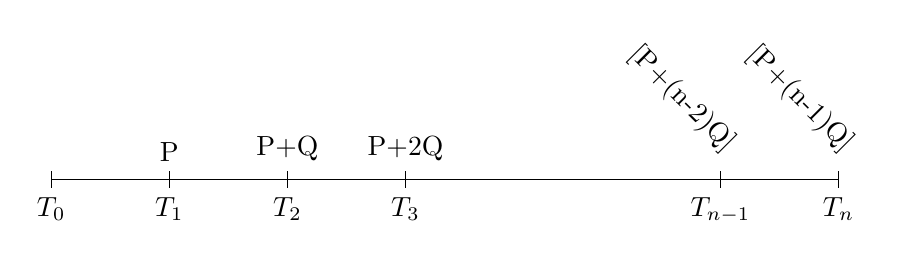
\begin{tikzpicture}
% draw horizontal line   
\draw (0,0) -- (10,0);

% draw vertical lines
\foreach \x in {0,1.5,3,4.5,8.5,10}
\draw (\x cm,3pt) -- (\x cm,-3pt);

% draw nodes
\draw (0,0) node[below=3pt] {$T_0$ } node[above=3pt] {};
\draw (1.5,0) node[below=3pt] {$T_1$} node[above=3pt] {P};
\draw (3,0) node[below=3pt] {$T_2$} node[above=3pt] {P+Q};
\draw (4.5,0) node[below=3pt] {$T_3$} node[above=3pt] {P+2Q};
\draw (8.5,0) node[below=3pt] {$T_{n-1}$} node[above=3pt, anchor= south east, rotate=-45] {[P+(n-2)Q]};
\draw (10,0) node[below=3pt] {$T_n$} node[above=3pt, anchor= south east, rotate=-45] {[P+(n-1)Q]};

\end{tikzpicture}

\vspace{30pt}As AboAmmar said, you could also rotate all the labels:

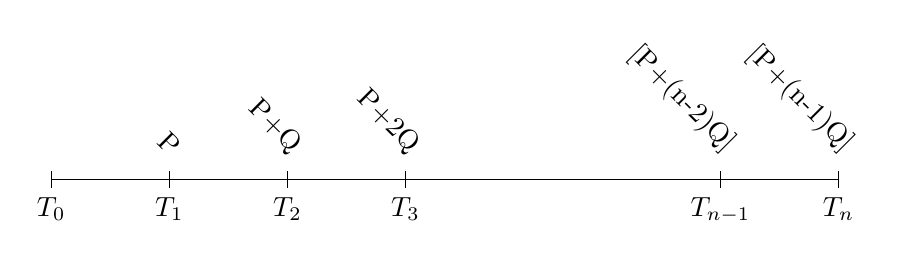
\begin{tikzpicture}[mylabel/.style={above=3pt, anchor= south east, rotate=-45}]
% draw horizontal line   
\draw (0,0) -- (10,0);

% draw vertical lines
\foreach \x in {0,1.5,3,4.5,8.5,10}
\draw (\x cm,3pt) -- (\x cm,-3pt);

% draw nodes
\draw (0,0) node[below=3pt] {$T_0$ } node[mylabel] {};
\draw (1.5,0) node[below=3pt] {$T_1$} node[mylabel] {P};
\draw (3,0) node[below=3pt] {$T_2$} node[mylabel] {P+Q};
\draw (4.5,0) node[below=3pt] {$T_3$} node[mylabel] {P+2Q};
\draw (8.5,0) node[below=3pt] {$T_{n-1}$} node[mylabel] {[P+(n-2)Q]};
\draw (10,0) node[below=3pt] {$T_n$} node[mylabel] {[P+(n-1)Q]};

\end{tikzpicture}
\end{document}